% !TeX program = xelatex
% 第十八章 极值与条件极值
\chapter{极值与条件极值}

本章讨论多元微分学的重要应用——多元函数的极值．回忆一元函数的极值问题，求解的基本思想是分两步走．第一步从函数定义域中确定出可能的极值点，第二步是判别这些可能的极值点是否确是极值点．为此，我们需要函数取极值的必要条件和充分条件．必要条件可以使我们实现第一步，而充分条件则可以实现第二步．对于多元函数的极值问题，我们仍然是按这样一条思路去做，分别给出函数取极值的必要条件和充分条件．不过对充分条件的讨论，多元函数情形要比一元函数情形复杂得多．

求条件极值的拉格朗日乘数法将条件极值完全化为了无条件极值，大大地简化了计算．

\section{极值与最小二乘法}

\subsection{多元函数的极值}

以二元函数为例进行讨论．

\begin{definition}\label{def:18-1}
设函数 $f(x,y)$ 在点 $P_{0}(x_{0},y_{0})$ 的某邻域 $O(P_{0})$ 内有定义．若对于任意点 $P(x,y)\in O(P_{0})$，有
\begin{equation}
f(P)\leqslant f(P_{0}),
\tag{1}
\end{equation}
则称函数 $f(x,y)$ 在 $P_{0}$ 点取极大值，点 $P_{0}$ 称为 $f$ 的极大值点．若对于任意点 $P\in O(P_{0})$，有 $f(P)\geqslant f(P_{0})$，则称函数 $f(x,y)$ 在 $P_{0}$ 取极小值，点 $P_{0}$ 称为 $f$ 的极小值点．
\end{definition}

极大值和极小值统称为极值．极大值点和极小值点统称为极值点．

从定义中易见，若 $P_{0}(x_{0},y_{0})$ 是 $f(x,y)$ 的极值点，则 $x_{0}$ 是一元函数 $f(x,y_{0})$ 的极值点，$y_{0}$ 是一元函数 $f(x_{0},y)$ 的极值点．而在 $P_{0}$ 点函数 $f(x,y)$ 的偏导数可能存在，也可能不存在．若是前者，则由一元函数取极值的必要条件便知，$f_{x}(x_{0},y_{0})=f_{y}(x_{0},y_{0})=0$．把这写成下面的定理．

\begin{theorem}[取极值的必要条件]\label{thm:18-1}
设函数 $f(x,y)$ 在点 $P_{0}(x_{0},y_{0})$ 存在对各变元的偏导数，且 $P_{0}$ 是极值点，则有
\begin{equation}
f_{x}(P_{0})=0,\quad f_{y}(P_{0})=0.
\tag{2}
\end{equation}
\end{theorem}

满足（2）式的点称为函数的稳定点．由定理 18.1 知，极值点要么是稳定点，要么在其上至少有一个偏导数不存在．

例如锥面 $z=\sqrt{x^{2}+y^{2}}$，显然它在点 $(0,0)$ 取得最小值，但在点 $(0,0)$ 两个偏导数 $z_{x}(0,0)$ 和 $z_{y}(0,0)$ 都不存在．参见图~\ref{fig:18-1}．

注意：定理 18.1 仅是取极值的必要条件，不是充分条件．例如马鞍面 $z=xy$ 在点 $(0,0)$ 有 $z_{x}(0,0)=z_{y}(0,0)=0$，但显然 $(0,0)$ 点不是极值点．事实上，在 $(0,0)$ 点的任何邻域内都存在两点其函数值异号，而 $z(0,0)=0$（见图~\ref{fig:18-2}）．

\begin{figure}[htbp]
\centering
\begin{minipage}[c]{0.42\textwidth}\centering
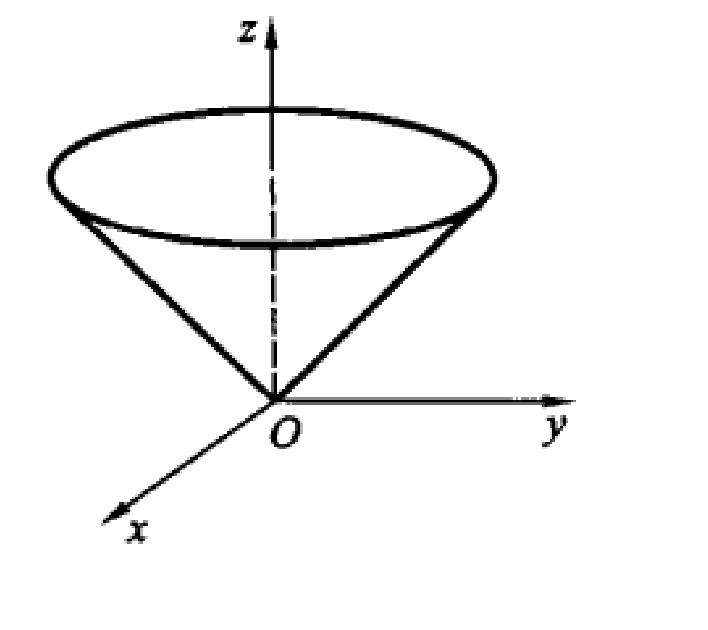
\includegraphics[width=0.86\textwidth]{work/figures/fig18-1}\caption{\relax}\label{fig:18-1}
\end{minipage}\hfill
\begin{minipage}[c]{0.55\textwidth}\centering
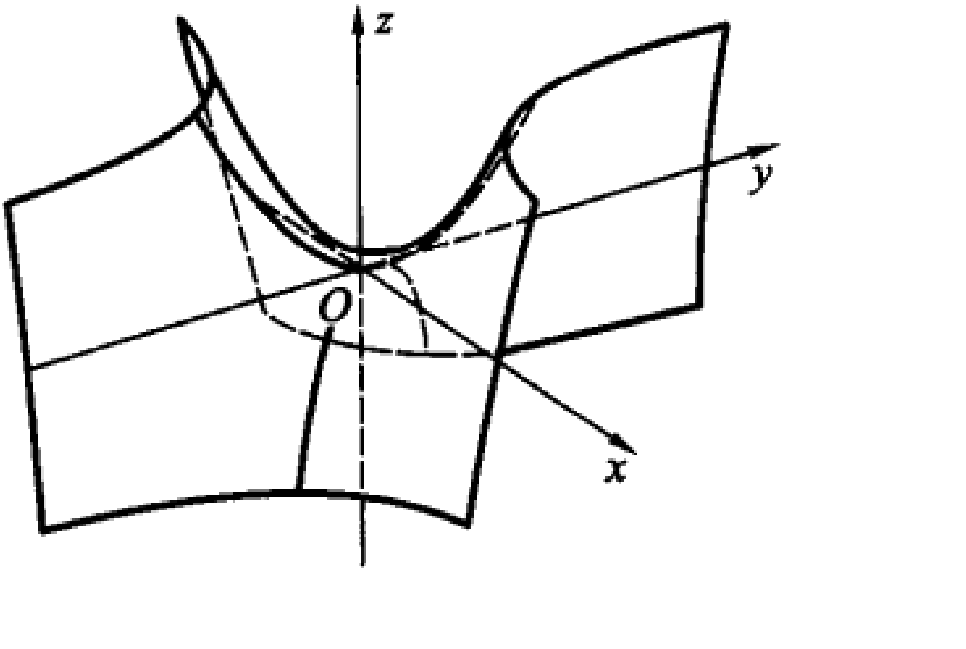
\includegraphics[width=0.98\textwidth]{work/figures/fig18-2}\caption{\relax}\label{fig:18-2}
\end{minipage}
\end{figure}

下面讨论取极值的充分条件，用来判别稳定点是否确是极值点．类似于一元函数的情形，我们用泰勒公式进行讨论．

设 $f(x,y)$ 在 $(x_{0},y_{0})$ 具有二阶连续偏导数．记
\[
a_{11}=f_{xx}(x_{0},y_{0}),\quad a_{12}=f_{xy}(x_{0},y_{0}),\quad a_{22}=f_{yy}(x_{0},y_{0}),
\]
\[
D=\left|\begin{array}{cc}a_{11}&a_{12}\\ a_{12}&a_{22}\end{array}\right|=a_{11}a_{22}-a_{12}^{2}.
\]

\begin{theorem}\label{thm:18-2}
如果 $f(x,y)$ 在 $P_{0}(x_{0},y_{0})$ 的某邻域内具有二阶的连续偏导数，$f_{x}(x_{0},y_{0})=0$，$f_{y}(x_{0},y_{0})=0$，那么

（i）若 $D>0$，则当 $a_{11}>0$（或 $a_{22}>0$）时，$f$ 在 $P_{0}$ 取极小值；当 $a_{11}<0$（或 $a_{22}<0$）时，$f$ 在 $P_{0}$ 取极大值．

（ii）若 $D<0$，则 $P_{0}$ 不是 $f$ 的极值点．

（iii）若 $D=0$，则不能判定 $f$ 在 $P_{0}$ 是否取极值，需进一步讨论．
\end{theorem}

\begin{proof}
用二元函数的泰勒公式，并注意到 $f_{x}(x_{0},y_{0})=0$，$f_{y}(x_{0},y_{0})=0$，则有
\[
\begin{aligned}
\Delta f&=f(x_{0}+\Delta x,y_{0}+\Delta y)-f(x_{0},y_{0})\\
&=\frac{1}{2}\left\{f_{xx}(x_{0}+\theta\Delta x,y_{0}+\theta\Delta y)\Delta x^{2}+2f_{xy}(x_{0}+\theta\Delta x,y_{0}+\theta\Delta y)\Delta x\Delta y+\right.\\
&\quad\left.f_{yy}(x_{0}+\theta\Delta x,y_{0}+\theta\Delta y)\Delta y^{2}\right\}\\
&=\frac{1}{2}\left\{f_{xx}(x_{0},y_{0})\Delta x^{2}+2f_{xy}(x_{0},y_{0})\Delta x\Delta y+f_{yy}(x_{0},y_{0})\Delta y^{2}+\right.\\
&\quad\left.\alpha_{11}\Delta x^{2}+2\alpha_{12}\Delta x\Delta y+\alpha_{22}\Delta y^{2}\right\}\\
&=\frac{1}{2}\left\{a_{11}\Delta x^{2}+2a_{12}\Delta x\Delta y+a_{22}\Delta y^{2}+\alpha_{11}\Delta x^{2}+2\alpha_{12}\Delta x\Delta y+\alpha_{22}\Delta y^{2}\right\},
\end{aligned}
\]
其中当 $\Delta x\to0$，$\Delta y\to0$ 时，
\[
\begin{aligned}
\alpha_{11}&=f_{xx}(x_{0}+\theta\Delta x,y_{0}+\theta\Delta y)-f_{xx}(x_{0},y_{0})\to0,\\
\alpha_{12}&=f_{xy}(x_{0}+\theta\Delta x,y_{0}+\theta\Delta y)-f_{xy}(x_{0},y_{0})\to0,\\
\alpha_{22}&=f_{yy}(x_{0}+\theta\Delta x,y_{0}+\theta\Delta y)-f_{yy}(x_{0},y_{0})\to0.
\end{aligned}
\]
为讨论方便，令 $\Delta x=\rho\cos\varphi$，$\Delta y=\rho\sin\varphi$，则
\[
\begin{aligned}
\Delta f&=\frac{\rho^{2}}{2}\left[a_{11}\cos^{2}\varphi+2a_{12}\cos\varphi\sin\varphi+a_{22}\sin^{2}\varphi+o(1)\right]\\
&=\frac{\rho^{2}}{2}\left[A(\varphi)+o(1)\right],
\end{aligned}
\]
其中 $o(1)$ 表示当 $\rho\to0$ 时的某个无穷小量．

（i）若 $D=a_{11}a_{22}-a_{12}^{2}>0$，则 $a_{11}\neq0$．这时
\begin{equation}
\begin{aligned}
A(\varphi)&=a_{11}\cos^{2}\varphi+2a_{12}\cos\varphi\sin\varphi+a_{22}\sin^{2}\varphi\\
&=\frac{1}{a_{11}}\left[\left(a_{11}\cos\varphi+a_{12}\sin\varphi\right)^{2}+\left(a_{11}a_{22}-a_{12}^{2}\right)\sin^{2}\varphi\right].
\end{aligned}
\tag{3}
\end{equation}
显然，对任意的 $\varphi$，$A(\varphi)$ 与 $a_{11}$ 同号．若 $a_{11}>0$，则 $A(\varphi)>0$．而 $A(\varphi)$ 是 $\varphi$ 的连续函数，因此
\[
m=\min_{0\leqslant\varphi\leqslant 2\pi}A(\varphi)>0,
\]
故存在 $\delta>0$，使得当 $\rho<\delta$ 时，$\left|o(1)\right|<m$，从而当 $\rho<\delta$ 时，$\Delta f$ 与 $A(\varphi)$ 同号，即 $\Delta f$ 与 $a_{11}$ 同号．于是证得，当 $a_{11}>0$ 时，$f$ 在 $P_{0}$ 取极小；同理，当 $a_{11}<0$ 时，$f$ 在 $P_{0}$ 取极大．注意到在这里 $x$ 与 $y$ 的地位是对称的，从而用 $a_{22}$ 代替 $a_{11}$ 可得类似的结论．

（ii）若 $D=a_{11}a_{22}-a_{12}^{2}<0$，这时分两种情形讨论．

第一种情形是 $a_{11}\neq0$，这时（3）式仍然成立．取 $\varphi=0$，则 $A(0)\neq0$，它与 $a_{11}$ 同号．取 $\rho$ 充分小，可使 $\Delta f$ 与 $A(0)$ 即与 $a_{11}$ 同号．取 $\varphi=\varphi_{1}$ 使 $a_{11}\cos\varphi_{1}+a_{12}\sin\varphi_{1}=0$，这时 $A(\varphi_{1})\neq0$，它与 $a_{11}$ 异号．取 $\rho$ 充分小，可使 $\Delta f$ 与 $A(\varphi_{1})$ 同号，从而 $\Delta f$ 与 $a_{11}$ 异号．这样，我们证明了，$\Delta f$ 在 $\varphi=0$ 与在 $\varphi=\varphi_{1}$ 是异号的（取 $\rho$ 充分小），也就是说，$f$ 在 $P_{0}$ 不取极值．

第二种情形是 $a_{11}=0$．这时 $a_{12}\neq0$，则
\[
A(\varphi)=\sin\varphi\left(2a_{12}\cos\varphi+a_{22}\sin\varphi\right).
\]
取 $\varphi=\varphi_{2}\neq0$，使
\[
\left|a_{22}\sin\varphi_{2}\right|<2\left|a_{12}\cos\varphi_{2}\right|,
\]
由 $a_{12}\neq0$ 这显然是办得到的．这样，当 $\varphi$ 分别取 $\varphi_{2}$ 与 $-\varphi_{2}$ 时，$A(\varphi)$ 取不同的符号，从而当 $\rho$ 充分小时，$\Delta f$ 取不同的符号．也就是说，$f$ 在 $P_{0}$ 不取极值．

（iii）若 $a_{11}a_{22}-a_{12}^{2}=0$，不能判定 $f$ 在 $P_{0}$ 是否取极值．例如函数 $f(x,y)=y^{2}+x^{3}$，$f(x,y)=(x^{2}+y^{2})^{2}$，在 $(0,0)$ 都有 $D=0$，但前者在 $(0,0)$ 不取极值，后者在 $(0,0)$ 取极小值．这时讨论需用更高阶的泰勒展开．定理 18.2 证完．
\end{proof}

定理 18.2 的证明思想是，通过二元函数的泰勒公式，得到
\[
\Delta f(x_{0},y_{0})=f(x_{0}+\Delta x,y_{0}+\Delta y)-f(x_{0},y_{0})=\frac{1}{2}\mathrm{d}^{2}f(x_{0},y_{0})+o(\rho^{2}).
\]
因此，若 $\mathrm{d}^{2}f(x_{0},y_{0})\neq0$，则当 $\rho$ 充分小时，$\Delta f(x_{0},y_{0})$ 与 $\mathrm{d}^{2}f(x_{0},y_{0})$ 同号．于是，若 $\mathrm{d}^{2}f(x_{0},y_{0})>0$，则 $P_{0}$ 是极小值点；若 $\mathrm{d}^{2}f(x_{0},y_{0})<0$，则 $P_{0}$ 是极大值点．又
\begin{equation}
\begin{aligned}
\mathrm{d}^{2}f(x_{0},y_{0})&=f_{xx}(x_{0},y_{0})\Delta x^{2}+2f_{xy}(x_{0},y_{0})\Delta x\Delta y+f_{yy}(x_{0},y_{0})\Delta y^{2}\\
&=\begin{pmatrix}\Delta x,\Delta y\end{pmatrix}
\begin{pmatrix}f_{xx}&f_{xy}\\ f_{xy}&f_{yy}\end{pmatrix}_{P_{0}}
\begin{pmatrix}\Delta x\\ \Delta y\end{pmatrix}=X^{\mathrm{T}}DX,
\end{aligned}
\tag{4}
\end{equation}
其中 $X=(\Delta x,\Delta y)^{\mathrm{T}}$．这是关于 $\Delta x$，$\Delta y$ 的二次型，由二次型理论，$X^{\mathrm{T}}DX>0$ 的充要条件是 $D$ 正定，而这又等价于 $A$ 的顺序主子式全大于零，故 $D>0$，且 $f_{xx}(x_{0},y_{0})>0$（或 $f_{yy}(x_{0},y_{0})>0$）时，$f(x,y)$ 在点 $P_{0}(x_{0},y_{0})$ 取极小值．而 $X^{\mathrm{T}}DX<0$ 的充要条件是 $D$ 负定，而这又等价于 $A$ 的顺序主子式负、正相间，故 $D>0$，且 $f_{xx}(x_{0},y_{0})<0$（或 $f_{yy}(x_{0},y_{0})<0$）时，$f(x,y)$ 在点 $P_{0}(x_{0},y_{0})$ 取极大值．若 $D<0$，则二次型 $\mathrm{d}^{2}f(x_{0},y_{0})=X^{\mathrm{T}}DX$ 是不定的．$\Delta f(x_{0},y_{0})$ 可正可负，也就是说函数在 $P_{0}(x_{0},y_{0})$ 不取极值．这种方法可以自然推广到更多个变量的情形．定理 18.2 的证明，实际上只是在两个自变量的情形，把 $\Delta f$ 与二次型同号，以及判别二次型正定的定理，都一起给出了证明．

根据上面的讨论有：若 $D$ 正定，即 $\mathrm{d}^{2}f(x_{0},y_{0})>0$，则 $f(x,y)$ 在点 $P_{0}(x_{0},y_{0})$ 取极小值；若 $D$ 负定，即 $\mathrm{d}^{2}f(x_{0},y_{0})<0$，则 $f(x,y)$ 在点 $P_{0}(x_{0},y_{0})$ 取极大值．反之，若 $f(x,y)$ 在点 $P_{0}(x_{0},y_{0})$ 取极小值，则 $D$ 半正定，即 $\mathrm{d}^{2}f(x_{0},y_{0})\geqslant0$；若 $f(x,y)$ 在点 $P_{0}(x_{0},y_{0})$ 取极大值，则 $D$ 半负定，即 $\mathrm{d}^{2}f(x_{0},y_{0})\leqslant0$．因此如果能直接验证 $\mathrm{d}^{2}f(x_{0},y_{0})>0$，也就可以断言 $f$ 在 $P_{0}(x_{0},y_{0})$ 取极小值．在下一节的例 2，我们将会看到这种情形．

\begin{example}\label{ex:18-1-1}
讨论函数 $z=f(x,y)=\dfrac{x^{2}}{2p}+\dfrac{y^{2}}{2q}$ $(p>0,q>0)$ 的极值．
\end{example}

\begin{proof}[解]
令
\[
\begin{cases}
\dfrac{\partial z}{\partial x}=\dfrac{x}{p}=0,\\[2mm]
\dfrac{\partial z}{\partial y}=\dfrac{y}{q}=0,
\end{cases}
\]
解得稳定点 $P_{0}(0,0)$．
\[
D=\left|\begin{array}{cc}a_{11}&a_{12}\\ a_{12}&a_{22}\end{array}\right|=\left|\begin{array}{cc}\dfrac{1}{p}&0\\[2mm] 0&\dfrac{1}{q}\end{array}\right|=\frac{1}{pq}>0,
\]
$a_{11}=\dfrac{1}{p}>0$，故 $P_{0}(0,0)$ 是 $f(x,y)$ 的极小值点．
\end{proof}

\subsection{最小二乘法}

极值的最重要的应用之一是最小二乘法，它是用实际测量的数据来拟合曲线的一种方法．

在现实生活中，常会遇到这样一类问题．两变量 $x$，$y$ 之间具有某种对应关系 $y=f(x)$，但并不知道 $f(x)$ 的准确表达式，我们希望通过实际的测量数据 $(x_{i},y_{i})$ $(i=1,2,\cdots,n)$，用一些简单、熟悉的曲线来近似它．多项式曲线比较简单，自然是最常采用的．一般来说先要对测量数据进行分析，如果它们大体上在一条直线上，便可用一次多项式即直线去近似它．我们仅以直线为例来说明这种近似方法或拟合方法．

我们知道两点可以唯一地确定一条通过这两点的直线．但仅用两点所含的信息量来反映 $x$，$y$ 之间的关系显然是不合理的，点数越多，所含的信息量就越多，而 $n(>2)$ 个点又如何确定一条直线呢？

设所求的拟合直线方程为 $y=ax+b$，$a$，$b$ 待定．在 $x_{i}$ 处，拟合直线取函数值 $ax_{i}+b$，而测量所得的函数值是 $y_{i}$，故
\[
\left|ax_{i}+b_{i}-y_{i}\right|
\]
给出在 $x_{i}$ 处拟合直线的值与测量值的误差．这个误差越小，说明拟合的效果在 $x_{i}$ 这点越准确．问题是这样的 $x_{i}$ 有 $n$ 个：$x_{1},x_{2},\cdots,x_{n}$．因此，刻画拟合的准确度应是这些误差的全体，即总误差．然而用什么来度量总误差？我们在第十四章 §4 即傅里叶级数的平均收敛性一节中就曾指出过，总误差可以有多种刻画，例如至少有下面的三种：
\[
\begin{aligned}
\rho_{1}&=\max_{1\leqslant i\leqslant n}\left|ax_{i}+b-y_{i}\right|,\\
\rho_{2}&=\sum_{i=1}^{n}\left|ax_{i}+b-y_{i}\right|,\\
\rho_{3}&=\sum_{i=1}^{n}\left(ax_{i}+b-y_{i}\right)^{2}.
\end{aligned}
\]

\begin{figure}[htbp]
\centering
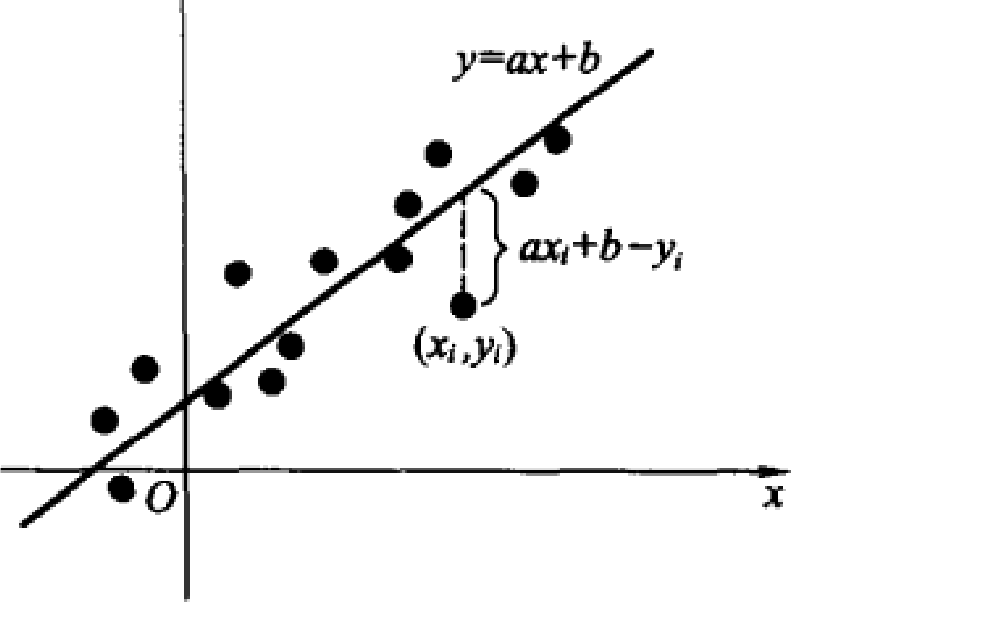
\includegraphics[width=0.42\textwidth]{work/figures/fig18-3}\caption{\relax}\label{fig:18-3}
\end{figure}

其中 $\rho_{1}$ 和 $\rho_{2}$ 由于绝对值的出现，用起来不大方便．而 $\rho_{3}$ 用乘方代替了 $\rho_{2}$ 中的绝对值，用起来就方便多了．这种使 $\rho_{3}$ 取最小即使所有点的误差的平方和取最小来确定拟合曲线的方法，就称为最小二乘法，它是由高斯（Gauss，1777—1855）首创的．在拟合曲线是直线的情形，最小二乘法就是确定 $a$，$b$，使 $\rho_{3}$ 达到最小．

记
\[
f(a,b)=\sum_{i=1}^{n}\left(ax_{i}+b-y_{i}\right)^{2}.
\]
为求其最小，分别对 $a$，$b$ 求偏导数，并令它们等于 $0$：
\[
\begin{aligned}
\frac{\partial f}{\partial a}&=2\sum_{i=1}^{n}\left(ax_{i}+b-y_{i}\right)x_{i}=0,\\
\frac{\partial f}{\partial b}&=2\sum_{i=1}^{n}\left(ax_{i}+b-y_{i}\right)=0,
\end{aligned}
\]
写出来就是
\[
\begin{cases}
\displaystyle a\sum_{i=1}^{n}x_{i}^{2}+b\sum_{i=1}^{n}x_{i}=\sum_{i=1}^{n}x_{i}y_{i},\\[3mm]
\displaystyle a\sum_{i=1}^{n}x_{i}+bn=\sum_{i=1}^{n}y_{i}.
\end{cases}
\]
为了把方程的解写清楚，记 $\bm{x}=(x_{1},x_{2},\cdots,x_{n})$，$\bm{y}=(y_{1},y_{2},\cdots,y_{n})$，$\bm{e}=(1,1,\cdots,1)$．引入内积
\[
(\bm{x},\bm{y})=\sum_{i=1}^{n}x_{i}y_{i},
\]
则上述方程组可以写为
\[
\begin{cases}
(\bm{x},\bm{x})a+(\bm{x},\bm{e})b=(\bm{x},\bm{y}),\\
(\bm{x},\bm{e})a+(\bm{e},\bm{e})b=(\bm{y},\bm{e}).
\end{cases}
\]
由克拉默法则，当 $\begin{vmatrix}(\bm{x},\bm{x})&(\bm{x},\bm{e})\\ (\bm{x},\bm{e})&(\bm{e},\bm{e})\end{vmatrix}\neq0$ 时，方程组有唯一解，这个解也是函数 $f$ 唯一的稳定点
\begin{equation}
\overline{a}=\frac{\begin{vmatrix}(\bm{x},\bm{y})&(\bm{x},\bm{e})\\ (\bm{y},\bm{e})&(\bm{e},\bm{e})\end{vmatrix}}{\begin{vmatrix}(\bm{x},\bm{x})&(\bm{x},\bm{e})\\ (\bm{x},\bm{e})&(\bm{e},\bm{e})\end{vmatrix}},\quad
\overline{b}=\frac{\begin{vmatrix}(\bm{x},\bm{x})&(\bm{x},\bm{y})\\ (\bm{x},\bm{e})&(\bm{y},\bm{e})\end{vmatrix}}{\begin{vmatrix}(\bm{x},\bm{x})&(\bm{x},\bm{e})\\ (\bm{x},\bm{e})&(\bm{e},\bm{e})\end{vmatrix}}.
\tag{5}
\end{equation}
由于函数 $f(a,b)$ 在全平面可微，且由实际问题知 $f$ 必有最小值，因此唯一的稳定点必是最小值点，即函数 $f(a,b)$ 在稳定点处取最小值．这样我们便求得拟合直线为
\[
y=\overline{a}x+\overline{b},
\]
其中，$\overline{a}$，$\overline{b}$ 由公式（5）给出．

最小二乘法也有它的不足之处．在测量中可能出现个别异常点，即与真实直线偏离较远的点，这时 $\left|y-y_{i}\right|$ 较大，平方后就更大．用平方和达到最小作标准，就可能导致拟合直线与真实直线偏离较大的情形（图~\ref{fig:18-4}）．从这个角度来说，$\rho_{2}$ 给出的总误差可以改善异常点带来的影响．对 $\rho_{2}$ 求最小来获得拟合直线的方法称为最小一乘法．

\begin{figure}[htbp]
\centering
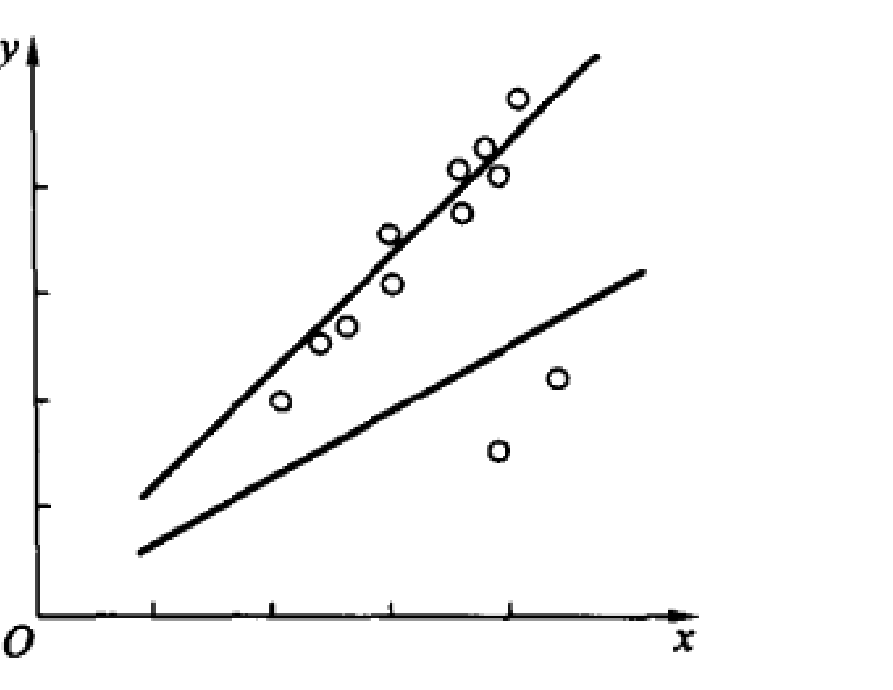
\includegraphics[width=0.4\textwidth]{work/figures/fig18-4}\caption{\relax}\label{fig:18-4}
\end{figure}

\subsection{多元函数的最值}

通过对最小二乘法的介绍，我们实际上已给出了一种利用极值求最值的方法．极值是函数 $f$ 在某点局部的性质，而最值是 $f$ 在某区域 $D$ 上的整体性质．只要搞清楚了最值与极值的关系，就可找到求最值的方法．

首先求出所有可能的最值点．函数 $f(x,y)$ 在 $D$ 上的最值点可能是 $D$ 的内点，也可能是 $D$ 的边界点．如果是 $D$ 的内点，则必是极值点．因此可能的最值点包括可能的极值点和属于 $D$ 的边界点．或者说可能的最值点就是稳定点、至少有一个偏导数不存在的点以及属于 $D$ 的边界点．

其次，我们来判别这些可能的最值点哪些是最大值点，哪些是最小值点．在已知 $f$ 于 $D$ 内存在最值的前提下，比较 $D$ 内所有可能的最值点的函数值（如果可能的话），就可确定出最大值点和最小值点．特别，若 $D$ 是开集，函数 $f$ 在 $D$ 内可导且稳定点唯一时，则唯一的稳定点就是最值点．值得指出的是，最值存在性的前提是重要的．例如马鞍面 $z=f(x,y)=xy$ 在单位圆 $D=\{(x,y)\mid x^{2}+y^{2}<1\}$ 内有唯一的稳定点 $(0,0)$，但这唯一的稳定点并不是最值点．

\begin{example}\label{ex:18-1-2}
试在 $x$ 轴，$y$ 轴与直线 $x+y=2\pi$ 围成的三角形区域上求函数 $u=\sin x+\sin y-\sin(x+y)$ 的最大值．
\end{example}

\begin{proof}[解]
所给区域为
\[
D=\left\{(x,y)\mid x+y\leqslant2\pi,x\geqslant0,y\geqslant0\right\}.
\]
函数 $u$ 在 $D$ 内可导，令
\[
\begin{cases}
\dfrac{\partial u}{\partial x}=\cos x-\cos(x+y)=0,\\[2mm]
\dfrac{\partial u}{\partial y}=\cos y-\cos(x+y)=0,
\end{cases}
\]
则有 $\cos x=\cos y$．当 $(x,y)$ 是 $D$ 的内点时必有 $x=y$，代入上式得
\[
\cos x-\cos 2x=\cos x-2\cos^{2}x+1=0,
\]
即
\[
(2\cos x+1)(1-\cos x)=0.
\]

\begin{figure}[htbp]
\centering
\begin{tikzpicture}[scale=0.8,baseline=(current bounding box.center)]
  % axes
  \draw[{-Latex}] (0,0) -- (4.3,0) node[below left] {$x$};
  \draw[{-Latex}] (0,0) -- (0,3.5) node[left] {$y$};
  \node[below left] at (0,0) {$O$};
  % shaded triangle
  \draw[pattern=north east lines] (0,0) -- (3.14,0) -- (0,3.14) -- cycle;
  % line x+y=2pi
  \draw[thick] (0,3.14) -- (3.14,0) node[midway,above,sloped] {$x+y=2\pi$};
  % tick labels
  \node[below] at (3.14,0) {$2\pi$};
  \node[left] at (0,3.14) {$2\pi$};
\end{tikzpicture}\caption{\relax}\label{fig:18-5}
\end{figure}

在 $D$ 的内部只有唯一的稳定点 $\left(\dfrac{2}{3}\pi,\dfrac{2}{3}\pi\right)$．函数 $u$ 在有界闭集 $D$ 上连续，故必存在最大值．比较边界上的函数值及稳定点的函数值：在稳定点的函数值 $u\left(\dfrac{2}{3}\pi,\dfrac{2}{3}\pi\right)=\dfrac{3}{2}\sqrt{3}$；在边界 $x=0$ 上，$u=0$；在边界 $y=0$ 上，$u=0$；在边界 $x+y=2\pi$ 上，
\[
u=\sin x+\sin y=\sin x+\sin(2\pi-x)=0.
\]
故最大值为 $\dfrac{3}{2}\sqrt{3}$，最大值点为 $\left(\dfrac{2}{3}\pi,\dfrac{2}{3}\pi\right)$．
\end{proof}

\begin{example}\label{ex:18-1-3}
证明 $t\geqslant1$，$s\geqslant0$ 时，$ts\leqslant t\ln t-t+\mathrm{e}^{s}$．
\end{example}

\begin{proof}
只要证 $f(s,t)=t\ln t-t+\mathrm{e}^{s}-ts$ 在 $D=\left\{(s,t)\mid s\geqslant0,t\geqslant1\right\}$ 上有最小值 $m\geqslant0$．令
\[
\begin{cases}
\dfrac{\partial f}{\partial s}=\mathrm{e}^{s}-t=0,\\[2mm]
\dfrac{\partial f}{\partial t}=\ln t-s=0,
\end{cases}
\]
解得 $\mathrm{e}^{s}=t$．这时有无穷多个稳定点，它们形成一条平面曲线．

下面我们用最小值的定义来说明稳定点是最小值点．固定 $t=t_{0}\geqslant1$，则有
\[
\frac{\partial f}{\partial s}<0,\ \text{当}\ 0\leqslant s<\ln t_{0}\ \text{时},
\]
\[
\frac{\partial f}{\partial s}>0,\ \text{当}\ \ln t_{0}<s\ \text{时},
\]

\begin{figure}[htbp]
\centering
\begin{tikzpicture}[scale=0.8,baseline=(current bounding box.center)]
  % axes: horizontal s, vertical t
  \draw[{-Latex}] (0,0) -- (4,0) node[below left] {$s$};
  \draw[{-Latex}] (0,0) -- (0,3.6) node[left] {$t$};
  \node[below left] at (0,0) {$O$};
  % curve t = e^s
  \draw[thick,domain=0:1.2,smooth,variable=\x] plot(\x,{exp(\x)});
  \node[right] at (1.2,{exp(1.2)}) {$t=\mathrm{e}^{s}$};
\end{tikzpicture}\caption{\relax}\label{fig:18-6}
\end{figure}

故在半直线 $t=t_{0}$ $(s\geqslant0)$ 上，$f$ 在 $(\ln t_{0},t_{0})$ 达到最小值．可见 $f$ 在 $D$ 上的最小值只能在曲线 $\mathrm{e}^{s}=t$ 上达到．但
\[
f(s,\mathrm{e}^{s})=\mathrm{e}^{s}s-\mathrm{e}^{s}+\mathrm{e}^{s}-\mathrm{e}^{s}s=0.
\]
从而有
\[
f(s,t)\geqslant0,\quad(s,t)\in D.
\]
\end{proof}

\begin{xiti}
\item 求下列函数的极大值点和极小值点：
\begin{ziti}
\item $f(x,y)=(x-y+1)^{2}$；
\item $f(x,y)=3axy-x^{3}-y^{3}$ $(a>0)$；
\item $f(x,y)=xy\sqrt{1-\dfrac{x^{2}}{a^{2}}-\dfrac{y^{2}}{b^{2}}}$ $(a,b>0)$；
\item $f(x,y)=\mathrm{e}^{2x}(x+y^{2}+2y)$；
\item $f(x,y)=\sin x+\cos y+\cos(x-y)$ $\left(0\leqslant x,y\leqslant\dfrac{\pi}{2}\right)$；
\item $f(x,y)=\left(\sqrt{x^{2}+y^{2}}-1\right)^{2}$．
\end{ziti}
\item 已知 $y=ax^{2}+bx+c$，观测得一组数据 $(x_{i},y_{i})$，$i=1,2,\cdots,n$，利用最小二乘法，求系数 $a$，$b$，$c$ 所满足的三元一次方程组．
\item 已知平面上 $n$ 个点的坐标分别是
\[
A_{1}(x_{1},y_{1}),A_{2}(x_{2},y_{2}),\cdots,A_{n}(x_{n},y_{n}),
\]
试求一点，使它与这 $n$ 个点距离的平方和最小．
\item 求下列函数在指定范围 $D$ 内的最大值和最小值：
\begin{ziti}
\item $f(x,y)=x^{2}-y^{2}$，$D=\left\{(x,y)\mid x^{2}+y^{2}\leqslant4\right\}$；
\item $f(x,y)=x^{2}-xy+y^{2}$，$D=\left\{(x,y)\mid\left|x\right|+\left|y\right|\leqslant1\right\}$；
\item $f(x,y,z)=(ax+by+cz)\mathrm{e}^{-(x^{2}+y^{2}+z^{2})}$，其中 $a^{2}+b^{2}+c^{2}>0$，$D=\mathbf{R}^{3}$．
\end{ziti}
\item 求证：
\begin{ziti}
\item $f(x,y)=Ax^{2}+2Bxy+Cy^{2}+2Dx+2Ey+F$ 在 $\mathbf{R}^{2}$ 有最小值，无最大值，其中 $A>0$，$B^{2}<AC$；
\item $f(x,y)=xy+\dfrac{1}{x}+\dfrac{1}{y}$ 在 $0<x$，$y<+\infty$ 有最小值，无最大值．
\end{ziti}
\item 设 $F(x,y,z)$ 有二阶连续偏导数，并且
\[
F(x_{0},y_{0},z_{0})=0,\quad F_{z}(x_{0},y_{0},z_{0})\neq0.
\]
讨论由 $F(x,y,z)=0$ 确定的隐函数 $z=f(x,y)$ 在 $(x_{0},y_{0})$ 取得极值的必要和充分条件．再求由
\[
x^{2}+y^{2}+z^{2}-2x+2y-4z-10=0
\]
所确定的 $z=f(x,y)$ 的极值．
\item 求下列隐函数的极大值和极小值：
\begin{ziti}
\item $(x+y)^{2}+(y+z)^{2}+(z+x)^{2}=3$；
\item $z^{2}+xyz-x^{2}-xy^{2}-9=0$．
\end{ziti}
\item 在已知周长为 $2p$ 的一切三角形中，求出面积为最大的三角形．
\item 有一块铁片，宽 $b=24\ \mathrm{cm}$，要把它的两边折起做成一个槽，使得容积最大，求每边的倾角 $\alpha$ 和折起的宽度 $x$（见下图）．

\begin{center}
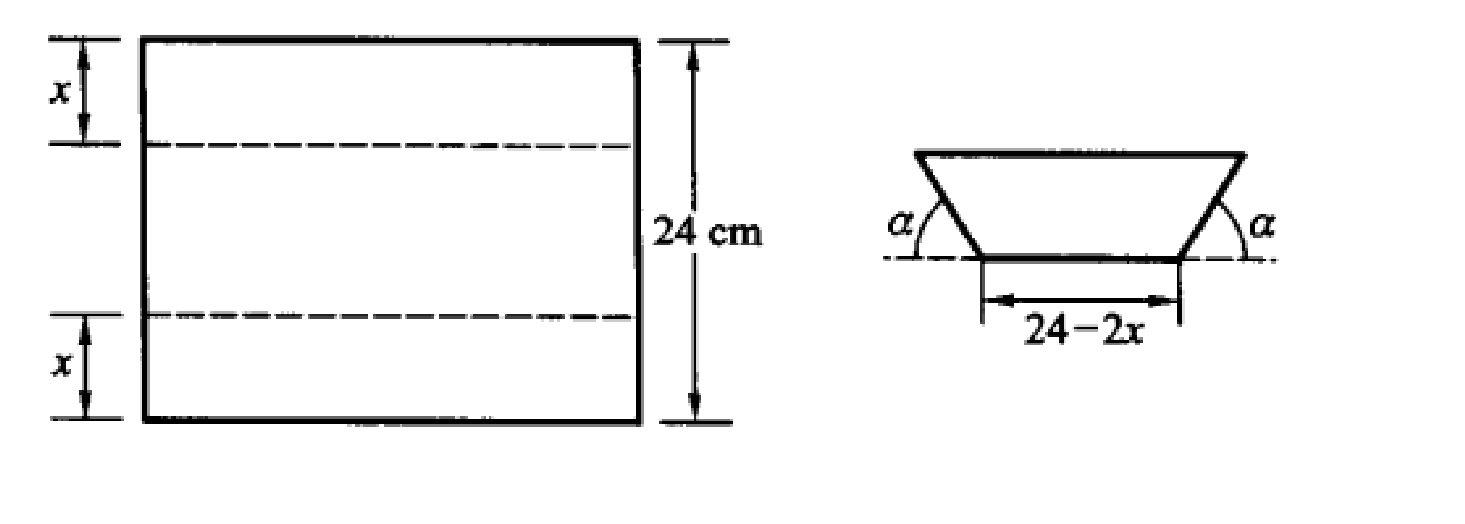
\includegraphics[width=0.66\textwidth]{work/figures/fig18-ex9}
\end{center}
\end{xiti}

\section{条件极值与拉格朗日乘数法}

前面我们考虑了函数 $f$ 在某区域 $D$ 上的极值问题．但实际问题中，函数 $f$ 的自变量不仅限制在某个区域上，它还可能受到其他条件的约束．例如，求单位球内截长方体，使其体积最大．如果取单位球面的方程 $x^{2}+y^{2}+z^{2}=1$，这时长方体的长、宽、高分别为 $2x$，$2y$，$2z$，因此长方体的体积为 $V=8xyz$．故抽象出来的数学问题是求目标函数
\[
V=8xyz
\]
满足约束条件
\[
\begin{cases}
x^{2}+y^{2}+z^{2}=1,\\
x,\quad y,\quad z>0
\end{cases}
\]
的最大值．这时函数 $V$ 的自变量 $x$，$y$，$z$ 不仅要满足定义域 $x$，$y$，$z>0$ 的要求，而且要满足条件 $x^{2}+y^{2}+z^{2}=1$．这类带有约束条件的极值问题就称为\emph{条件极值}问题．而前面讨论的不带约束条件的极值问题就称为无条件极值或普通极值问题．

条件极值有时可以化为无条件极值来求解．比如上面的条件极值问题，从球面方程中可解出 $z=\sqrt{1-x^{2}-y^{2}}$，代入目标函数，则问题等价于求
\[
V=8xy\sqrt{1-x^{2}-y^{2}}
\]
在区域 $D=\left\{(x,y)\mid x^{2}+y^{2}\leqslant1,x\geqslant0,y\geqslant0\right\}$ 的无条件极值．

条件极值问题的一般形式为求目标函数
\[
y=f(x_{1},x_{2},\cdots,x_{n})
\]
在约束条件
\[
g_{k}(x_{1},x_{2},\cdots,x_{n})=0,\quad k=1,2,\cdots,m\ (m<n)
\]
下的极值．

也就是说，约束方程可以有多个，而且它们可能对各变量来说都是隐式．这时要从约束条件方程组中解出 $m$ 个显函数是非常困难甚至是不可能的．因此，希望寻求一种无需解出显函数来的方法．我们讨论 $n=4$，$m=2$ 这种较简单的情形，但方法已具有一般性．这时是要求目标函数 $f(x,y,u,v)$ 在约束条件
\begin{equation}
\begin{cases}
F(x,y,u,v)=0,\\
G(x,y,u,v)=0
\end{cases}
\tag{1}
\end{equation}
下的条件极值，其中 $(x,y,u,v)\in U$．

以极小值为例，称点 $P_{0}(x_{0},y_{0},u_{0},v_{0})$ 是函数 $f$ 在条件（1）下的极小值点，如果 $P_{0}$ 满足（1）式，且存在 $P_{0}$ 点的某邻域 $O(P_{0})\subset U$，使得对任意满足（1）式的 $P(x,y,u,v)\in O(P_{0})$，有
\begin{equation}
f(x,y,u,v)\geqslant f(x_{0},y_{0},u_{0},v_{0}).
\tag{2}
\end{equation}
为了能用微分学来进行研究，假设 $f$，$F$，$G$ 在 $U$ 内具有对各变元的连续偏导数．我们主要考虑取极值的必要条件．

设点 $P_{0}(x_{0},y_{0},u_{0},v_{0})$ 是函数 $f$ 在条件（1）下的极值点，则
\begin{equation}
F(P_{0})=G(P_{0})=0,
\tag{3}
\end{equation}
且（2）式成立．如果 $\left.\dfrac{\partial(F,G)}{\partial(u,v)}\right|_{P_{0}}\neq0$，那么由隐函数组存在定理知，在 $P_{0}$ 点的某邻域内，方程组（1）唯一地确定一组可微函数
\[
\begin{cases}
u=u(x,y),\\
v=v(x,y),
\end{cases}
\]
它定义在 $(x_{0},y_{0})$ 的某邻域 $D$ 内，当 $(x,y)\in D$ 时，$(x,y,u,v)\in U$，且这组函数满足方程组（1）和
\[
u_{0}=u(x_{0},y_{0}),\ v_{0}=(x_{0},y_{0}).
\]
这时（2）式等价于说，$(x_{0},y_{0})$ 是函数
\[
g(x,y)=f(x,y,u(x,y),v(x,y))
\]
的无条件极值点．由无条件极值的必要条件知，$(x_{0},y_{0})$ 必须满足
\begin{equation}
\mathrm{d}g(x_{0},y_{0})=\left\{\frac{\partial f}{\partial x}\mathrm{d}x+\frac{\partial f}{\partial y}\mathrm{d}y+\frac{\partial f}{\partial u}\mathrm{d}u+\frac{\partial f}{\partial v}\mathrm{d}v\right\}_{(x_{0},y_{0})}=0.
\tag{4}
\end{equation}
注意这里 $\mathrm{d}x$，$\mathrm{d}y$，$\mathrm{d}u$，$\mathrm{d}v$ 不是独立的，它们在 $P_{0}(x_{0},y_{0},u_{0},v_{0})$ 满足
\begin{align}
\mathrm{d}F(P_{0})&=\left\{\frac{\partial F}{\partial x}\mathrm{d}x+\frac{\partial F}{\partial y}\mathrm{d}y+\frac{\partial F}{\partial u}\mathrm{d}u+\frac{\partial F}{\partial v}\mathrm{d}v\right\}_{P_{0}}=0,
\tag{5}\\
\mathrm{d}G(P_{0})&=\left\{\frac{\partial G}{\partial x}\mathrm{d}x+\frac{\partial G}{\partial y}\mathrm{d}y+\frac{\partial G}{\partial u}\mathrm{d}u+\frac{\partial G}{\partial v}\mathrm{d}v\right\}_{P_{0}}=0.
\tag{6}
\end{align}
将（5）式（6）式分别乘以 $\lambda_{1}$ 和 $\lambda_{2}$ 后与（4）式一起相加得
\begin{equation}
\begin{aligned}
\bigg\{\left(\frac{\partial f}{\partial x}+\lambda_{1}\frac{\partial F}{\partial x}+\lambda_{2}\frac{\partial G}{\partial x}\right)&\mathrm{d}x+\left(\frac{\partial f}{\partial y}+\lambda_{1}\frac{\partial F}{\partial y}+\lambda_{2}\frac{\partial G}{\partial y}\right)\mathrm{d}y+\\
\left(\frac{\partial f}{\partial u}+\lambda_{1}\frac{\partial F}{\partial u}+\lambda_{2}\frac{\partial G}{\partial u}\right)&\mathrm{d}u+\left(\frac{\partial f}{\partial v}+\lambda_{1}\frac{\partial F}{\partial v}+\lambda_{2}\frac{\partial G}{\partial v}\right)\mathrm{d}v\bigg\}_{P_{0}}=0,
\end{aligned}
\tag{7}
\end{equation}
其中 $\lambda_{1}$，$\lambda_{2}$ 待定．由于 $\mathrm{d}x$，$\mathrm{d}y$，$\mathrm{d}u$，$\mathrm{d}v$ 不独立，故不能从（7）推出 $\mathrm{d}x$，$\mathrm{d}y$，$\mathrm{d}u$，$\mathrm{d}v$ 的系数等于零．但已知 $\left.\dfrac{\partial(F,G)}{\partial(u,v)}\right|_{P_{0}}\neq0$，故方程组
\[
\begin{cases}
\dfrac{\partial f}{\partial u}+\lambda_{1}\dfrac{\partial F}{\partial u}+\lambda_{2}\dfrac{\partial G}{\partial u}=0,\\[2mm]
\dfrac{\partial f}{\partial v}+\lambda_{1}\dfrac{\partial F}{\partial v}+\lambda_{2}\dfrac{\partial G}{\partial v}=0
\end{cases}
\]
在 $P_{0}$ 点有唯一解 $(\lambda_{1},\lambda_{2})$，这时（7）式化为
\[
\left\{\left(\frac{\partial f}{\partial x}+\lambda_{1}\frac{\partial F}{\partial x}+\lambda_{2}\frac{\partial G}{\partial x}\right)\mathrm{d}x+\left(\frac{\partial f}{\partial y}+\lambda_{1}\frac{\partial F}{\partial y}+\lambda_{2}\frac{\partial G}{\partial y}\right)\mathrm{d}y\right\}_{P_{0}}=0.
\]
由于 $\mathrm{d}x$，$\mathrm{d}y$ 独立，则它们的系数等于零，于是得 $P_{0}$ 及 $(\lambda_{1},\lambda_{2})$ 所满足的方程组
\[
\begin{aligned}
\frac{\partial f}{\partial x}+\lambda_{1}\frac{\partial F}{\partial x}+\lambda_{2}\frac{\partial G}{\partial x}&=0,\\
\frac{\partial f}{\partial y}+\lambda_{1}\frac{\partial F}{\partial y}+\lambda_{2}\frac{\partial G}{\partial y}&=0,\\
\frac{\partial f}{\partial u}+\lambda_{1}\frac{\partial F}{\partial u}+\lambda_{2}\frac{\partial G}{\partial u}&=0,\\
\frac{\partial f}{\partial v}+\lambda_{1}\frac{\partial F}{\partial v}+\lambda_{2}\frac{\partial G}{\partial v}&=0,\\
F(x,y,u,v)&=0,\\
G(x,y,u,v)&=0.
\end{aligned}
\]
方程组含 $6$ 个方程，$6$ 个未知数 $(x,y,u,v,\lambda_{1},\lambda_{2})$，一般说来是可以由此解出 $(x_{0},y_{0},u_{0},v_{0})$ 和 $(\lambda_{1},\lambda_{2})$ 的．这时 $(x_{0},y_{0},u_{0},v_{0})$ 就是 $f(x,y,u,v)$ 在条件（1）下的稳定点，而 $(x_{0},y_{0})$ 就是函数 $g(x,y)$ 的无条件极值的稳定点．

引入辅助函数
\begin{equation}
L(x,y,u,v)=f(x,y,u,v)+\lambda_{1}F(x,y,u,v)+\lambda_{2}G(x,y,u,v),
\tag{8}
\end{equation}
则上述方程组前四个式子恰为
\[
L_{x}(P_{0})=L_{y}(P_{0})=L_{u}(P_{0})=L_{v}(P_{0})=0.
\]
（8）式定义的函数称为拉格朗日函数，而 $\lambda_{1}$，$\lambda_{2}$ 称为拉格朗日乘数．上面的讨论即是说：若 $P_{0}(x_{0},y_{0},u_{0},v_{0})$ 是函数 $f$ 在条件（1）下的条件极值点，则 $P_{0}$ 是拉格朗日函数的稳定点，且 $P_{0}$ 满足约束条件（1）．我们把上面的推理总结为下面的定理．

\begin{theorem}\label{thm:18-3}
若 $f(x,y,u,v)$，$F(x,y,u,v)$，$G(x,y,u,v)$ 在点 $P_{0}(x_{0},y_{0},$ $u_{0},v_{0})$ 的某邻域有连续的偏导数，且函数 $f$ 在约束条件（1）下在 $P_{0}$ 点取极值，矩阵
\begin{equation}
\left.\begin{pmatrix}F_{x}&F_{y}&F_{u}&F_{v}\\ G_{x}&G_{y}&G_{u}&G_{v}\end{pmatrix}\right|_{P_{0}}
\tag{9}
\end{equation}
的秩为 $2$，则存在唯一确定的 $\lambda_{1},\lambda_{2}$，使得
\begin{equation}
\begin{cases}
L_{x}(P_{0})=L_{y}(P_{0})=L_{u}(P_{0})=L_{v}(P_{0})=0,\\
F(P_{0})=G(P_{0})=0,
\end{cases}
\tag{10}
\end{equation}
其中 $L(x,y,u,v)$ 是拉格朗日函数，其定义为 $L=f+\lambda_{1}F+\lambda_{2}G$．
\end{theorem}

注意（10）式中有六个方程，由它可以确定六个未知数 $(x_{0},y_{0},u_{0},v_{0})$ 和 $\lambda_{1}$，$\lambda_{2}$．其中 $(x_{0},y_{0},u_{0},v_{0})$ 是拉格朗日函数的稳定点，从而是函数 $f(x,y,u,v)$ 的可能条件极值点，而 $(x_{0},y_{0})$ 就是函数 $g(x,y)$ 的可能无条件极值点．又因为 $(x_{0},y_{0},u_{0},v_{0})$ 是 $f(x,y,u,v)$ 的条件极值点等价于 $(x_{0},y_{0})$ 是 $g(x,y)$ 的无条件极值点，故只要用无条件极值的充分条件即可判别稳定点 $(x_{0},y_{0},u_{0},v_{0})$ 是否为 $f$ 的条件极值点．

值得指出的是，我们用矩阵（9）的秩为 $2$ 代替了条件 $\left.\dfrac{\partial(F,G)}{\partial(u,v)}\right|_{P_{0}}\neq0$，其理由是，由（9）的秩为 $2$ 知总有一个二阶行列式不为零，对此进行类似于上述的推理，便得到一样的结果．读者应注意到所有变量 $x$，$y$，$u$，$v$ 在方程组（10）中的位置是对等的．

现在我们回头来解本节开头提出的问题：求 $V=8xyz$ 满足约束条件
\[
x^{2}+y^{2}+z^{2}=1,\ x,y,z>0
\]
的最大值．

作拉格朗日函数
\[
L(x,y,z)=8xyz+\lambda(x^{2}+y^{2}+z^{2}-1).
\]
令
\[
\begin{aligned}
L_{x}&=8yz+2\lambda x=0,\\
L_{y}&=8xz+2\lambda y=0,\\
L_{z}&=8xy+2\lambda z=0,\\
x^{2}+y^{2}+z^{2}&=1.
\end{aligned}
\]
由前三式及 $x>0$，$y>0$，$z>0$ 得
\[
8xyz=-2\lambda x^{2}=-2\lambda y^{2}=-2\lambda z^{2},
\]
从而 $x=y=z$，代入最后一式得
\[
3x^{2}=1,
\]
解得拉格朗日函数的稳定点为
\[
x=y=z=\frac{1}{\sqrt{3}}.
\]
由实际问题知所求最大值必存在，而稳定点又唯一，因此唯一的稳定点就是最大值点．故球内截长方体中以正方体的体积为最大．

\begin{example}\label{ex:18-2-1}
求 $f(x,y,z)=xyz$ 在条件 $\dfrac{1}{x}+\dfrac{1}{y}+\dfrac{1}{z}=\dfrac{1}{r}$ $(x>0,y>0,z>0,r>0)$ 下的极小值；并证明不等式
\[
3\left(\frac{1}{x}+\frac{1}{y}+\frac{1}{z}\right)^{-1}\leqslant\sqrt[3]{xyz},
\]
其中 $x$，$y$，$z$ 为任意正实数．
\end{example}

\begin{proof}[解]
作拉格朗日函数
\[
L(x,y,z)=xyz+\lambda\left(\frac{1}{x}+\frac{1}{y}+\frac{1}{z}-\frac{1}{r}\right).
\]
令
\[
\begin{cases}
L_{x}=yz-\dfrac{\lambda}{x^{2}}=0,\\[2mm]
L_{y}=xz-\dfrac{\lambda}{y^{2}}=0,\\[2mm]
L_{z}=xy-\dfrac{\lambda}{z^{2}}=0,\\[2mm]
\dfrac{1}{x}+\dfrac{1}{y}+\dfrac{1}{z}=\dfrac{1}{r}.
\end{cases}
\]
由前三式得
\[
xyz=\frac{\lambda}{x}=\frac{\lambda}{y}=\frac{\lambda}{z}.
\]
因此，$x=y=z$．把它代入最后一式即得拉格朗日函数的稳定点为
\[
x=y=z=3r.
\]
下面判别稳定点是极值点．若记 $F(x,y,z)=\dfrac{1}{x}+\dfrac{1}{y}+\dfrac{1}{z}-\dfrac{1}{r}$，则 $F_{z}(3r,$ $3r,3r)=-\left.\dfrac{1}{z^{2}}\right|_{z=3r}\neq0$．故方程
\[
\frac{1}{x}+\frac{1}{y}+\frac{1}{z}=\frac{1}{r}
\]
在稳定点的附近可唯一地确定可微函数 $z=z(x,y)$．令
\[
g(x,y)=f(x,y,z(x,y)),
\]
我们用二元函数取无条件极值的充分条件判别 $(3r,3r)$ 是 $g(x,y)$ 的极值点．由约束条件得
\[
\frac{\partial z}{\partial x}=-\frac{z^{2}}{x^{2}},\quad\frac{\partial z}{\partial y}=-\frac{z^{2}}{y^{2}}.
\]
由复合函数链式法则
\[
\begin{aligned}
\frac{\partial g}{\partial x}&=yz+xy\frac{\partial z}{\partial x}=yz-\frac{yz^{2}}{x},\\
\frac{\partial g}{\partial y}&=xz+xy\frac{\partial z}{\partial y}=xz-\frac{xz^{2}}{y},\\
\frac{\partial^{2}g}{\partial x^{2}}&=y\frac{\partial z}{\partial x}+\frac{yz^{2}}{x^{2}}-\frac{2yz}{x}\frac{\partial z}{\partial x}=\frac{2yz^{3}}{x^{3}},\\
\frac{\partial^{2}g}{\partial x\partial y}&=z+y\frac{\partial z}{\partial y}-\frac{z^{2}}{x}-\frac{2yz}{x}\frac{\partial z}{\partial y}=z-\frac{z^{2}}{y}-\frac{z^{2}}{x}+\frac{2z^{3}}{xy},\\
\frac{\partial^{2}g}{\partial y^{2}}&=\frac{2xz^{3}}{y^{3}}.
\end{aligned}
\]
故函数 $g$ 在 $(3r,3r)$ 点有
\[
\left|\begin{array}{cc}a_{11}&a_{12}\\ a_{12}&a_{22}\end{array}\right|=\left|\begin{array}{cc}6r&3r\\ 3r&6r\end{array}\right|=36r^{2}-9r^{2}=27r^{2}>0,
\]
且 $a_{11}=6r>0$．因此 $g(x,y)$ 在 $(3r,3r)$ 处取极小值，这等价于 $f(x,y,z)$ 在 $(3r,3r,3r)$ 处取条件极小值
\[
f(3r,3r,3r)=(3r)^{3}.
\]
分析约束集 $D$：
\[
D=\left\{(x,y,z)\mid\frac{1}{x}+\frac{1}{y}+\frac{1}{z}=\frac{1}{r},\ x>0,y>0,z>0\right\},
\]
它是一无界集，当 $(x,y,z)$ 在 $D$ 内远离坐标原点时，函数 $f$ 将趋于正无穷．因此，函数 $f$ 的唯一极小值点是函数的最小值点，即有
\[
xyz\geqslant(3r)^{3},\quad(x,y,z)\in D.
\]
由于在 $D$ 内有 $r=\left(\dfrac{1}{x}+\dfrac{1}{y}+\dfrac{1}{z}\right)^{-1}$，代入上式即得
\[
3\left(\frac{1}{x}+\frac{1}{y}+\frac{1}{z}\right)^{-1}\leqslant\sqrt[3]{xyz},\ x,y,z>0.
\]
注意上式又可写为
\[
\sqrt[3]{\frac{1}{xyz}}\leqslant\frac{\dfrac{1}{x}+\dfrac{1}{y}+\dfrac{1}{z}}{3},
\]
这就是我们熟悉的平均值不等式：三个正实数 $\dfrac{1}{x}$，$\dfrac{1}{y}$，$\dfrac{1}{z}$ 的几何平均与算术平均的关系．
\end{proof}

\begin{example}\label{ex:18-2-2}
求函数 $f=x+y+z+t$ 在约束条件 $xyzt=c^{4}$（其中 $x,y,z,t,c>0$）下的极值．
\end{example}

\begin{proof}[解]
作拉格朗日函数
\[
L(x,y,z,t)=x+y+z+t+\lambda(xyzt-c^{4}).
\]
令
\[
\begin{cases}
L_{x}=1+\lambda yzt=0,\\
L_{y}=1+\lambda xzt=0,\\
L_{z}=1+\lambda xyt=0,\\
L_{t}=1+\lambda xyz=0,\\
xyzt=c^{4}.
\end{cases}
\]
由前四式得
\[
-\lambda xyzt=x=y=z=t\ \text{；}
\]
再从最后一式解得稳定点
\[
x=y=z=t=c.
\]
下面判定稳定点是极值点．注意此例中函数 $f$ 有 $4$ 个自变量，但只有一个约束条件．由约束条件确定出某个隐函数代入 $f$ 后，则 $f$ 还有 $3$ 个独立的自变量，因此不能类似上例用定理 18.2 来判别．为此我们用 $\mathrm{d}^{2}f(c,c,c,c)$ 的符号来判别是否极值．

在求微分之前，我们必须搞清楚变量之间的关系．由于有一个约束条件 $xyzt=c^{4}$，变量 $x$，$y$，$z$，$t$ 之间不是独立的，从而 $\mathrm{d}x$，$\mathrm{d}y$，$\mathrm{d}z$，$\mathrm{d}t$ 之间也不是独立的．它们之间的关系可以通过在约束条件等式两边求微分而得到：
\begin{equation}
yzt\mathrm{d}x+xzt\mathrm{d}y+xyt\mathrm{d}z+xyz\mathrm{d}t=0.
\tag{11}
\end{equation}
特别在稳定点 $(c,c,c,c)$ 处 $\mathrm{d}x,\mathrm{d}y,\mathrm{d}z,\mathrm{d}t$ 应满足
\begin{equation}
\mathrm{d}x+\mathrm{d}y+\mathrm{d}z+\mathrm{d}t=0.
\tag{12}
\end{equation}
也就是说，四个变量中只有三个是独立变量．这里不妨取 $x$，$y$，$z$ 为独立变量，则 $t$ 是 $x$，$y$，$z$ 的函数，那么（11）（12）式中 $\mathrm{d}x$，$\mathrm{d}y$，$\mathrm{d}z$ 是自变量的微分，而 $\mathrm{d}t$ 是函数的微分．这时 $f=f(x,y,z,t(x,y,z))$．

明确了上述变量之间的关系后，我们来求微分．由一阶微分形式不变性有
\[
\mathrm{d}f=\mathrm{d}x+\mathrm{d}y+\mathrm{d}z+\mathrm{d}t,
\]
其中 $\mathrm{d}x,\mathrm{d}y,\mathrm{d}z,\mathrm{d}t$ 满足（11）式，从而
\[
\mathrm{d}^{2}f=\mathrm{d}^{2}t.
\]
为求 $\mathrm{d}^{2}t$，在（11）式两边再求微分，得
\[
\begin{aligned}
&\left(zt\mathrm{d}y+yt\mathrm{d}z+yz\mathrm{d}t\right)\mathrm{d}x+\left(zt\mathrm{d}x+xt\mathrm{d}z+xz\mathrm{d}t\right)\mathrm{d}y+\\
&\left(yt\mathrm{d}x+xt\mathrm{d}y+xy\mathrm{d}t\right)\mathrm{d}z+\left(yz\mathrm{d}x+xz\mathrm{d}y+xy\mathrm{d}z\right)\mathrm{d}t+\\
&xyz\mathrm{d}^{2}t=0,
\end{aligned}
\]
在上式中令 $x=y=z=t=c$，得
\[
\mathrm{d}^{2}t=\frac{-2}{c}\left[\mathrm{d}x\mathrm{d}y+\mathrm{d}y\mathrm{d}z+\mathrm{d}x\mathrm{d}z+\mathrm{d}t\left(\mathrm{d}x+\mathrm{d}y+\mathrm{d}z\right)\right],
\]
其中 $\mathrm{d}x,\mathrm{d}y,\mathrm{d}z,\mathrm{d}t$ 满足（12）式，将（12）式代入得
\[
\begin{aligned}
\mathrm{d}^{2}t&=-\frac{2}{c}\left[\mathrm{d}x\mathrm{d}y+\mathrm{d}y\mathrm{d}z+\mathrm{d}x\mathrm{d}z-\left(\mathrm{d}x+\mathrm{d}y+\mathrm{d}z\right)^{2}\right]\\
&=\frac{1}{c}\left[\left(\mathrm{d}x+\mathrm{d}y+\mathrm{d}z\right)^{2}+\mathrm{d}x^{2}+\mathrm{d}y^{2}+\mathrm{d}z^{2}\right]>0,
\end{aligned}
\]
即
\[
\left.\mathrm{d}^{2}f\right|_{(c,c,c,c)}>0.
\]
因此函数 $f$ 在 $(c,c,c,c)$ 取条件极小值，$f(c,c,c,c)=4c$．
\end{proof}

前面我们已经看到，利用拉格朗日函数 $L(P)$，使我们可以方便地求得可能的条件极值点．其实，利用拉格朗日函数 $L(P)$ 还可以判别可能的极值点是否确是极值点，即有下述结论：

设 $P_{0}$ 是拉格朗日函数的稳定点，则

（1）若 $\mathrm{d}^{2}L(P_{0})>0$，则 $f$ 在 $P_{0}$ 取条件极小；

（2）若 $\mathrm{d}^{2}L(P_{0})<0$，则 $f$ 在 $P_{0}$ 取条件极大．我们把证明留给读者（习题 11）．

这个结论和必要条件（定理 18.3）一起表明，拉格朗日函数使条件极值问题完全化为了无条件极值．它消除了约束条件的影响，使所有变量处于平等地位．这个方法是拉格朗日引进的，称为拉格朗日乘数法，它简明优美，可算应用数学的一个典范．

\begin{xiti}
\item 求下列函数在所给条件下的极值：
\begin{ziti}
\item $f=x+y$，若 $x^{2}+y^{2}=1$；
\item $f=x^{2}+y^{2}$，若 $x+y-1=0$；
\item $f=x-2y+2z$，若 $x^{2}+y^{2}+z^{2}=1$；
\item $f=\dfrac{1}{x}+\dfrac{1}{y}$，若 $x+y=2$；
\item $f=xyz$，若 $x^{2}+y^{2}+z^{2}=1$，$x+y+z=0$；
\item $f=ax^{2}+by^{2}+2hxy$，若 $x^{2}+y^{2}=1$；
\item $f=x^{2}+y^{2}+z^{2}$，若 $(x^{2}+y^{2}+z^{2})^{2}=a^{2}x^{2}+b^{2}y^{2}+c^{2}z^{2}$，$lx+my+nz=0$．
\end{ziti}
\item 求 $f=x^{m}y^{n}z^{p}$ 在条件 $x+y+z=a$，$a>0$，$m>0$，$n>0$，$p>0$，$x>0$，$y>0$，$z>0$ 之下的最大值．
\item 求函数 $z=\dfrac{1}{2}(x^{n}+y^{n})$ 在条件 $x+y=l$ $(l>0,n\geqslant1)$ 之下的极值，并证明：当 $a\geqslant0$，$b\geqslant0$，$n\geqslant1$ 时
\[
\left(\frac{a+b}{2}\right)^{n}\leqslant\frac{a^{n}+b^{n}}{2}.
\]
\item 求表面积一定而体积最大的长方体．
\item 求体积一定而表面积最小的长方体．
\item 求圆的外切三角形中面积最小者．
\item 长为 $a$ 的铁丝切成两段，一段围成正方形，另一段围成圆．这两段的长各为多少时，它们所围正方形面积和圆面积之和最小．
\item 求原点到二平面 $a_{1}x+b_{1}y+c_{1}z+d_{1}=0$，$a_{2}x+b_{2}y+c_{2}z+d_{2}=0$ 的交线的最短距离．
\item 求抛物线 $y=x^{2}$ 和直线 $x-y=1$ 间的最短距离．
\item 求 $x>0$，$y>0$，$z>0$ 时函数 $f(x,y,z)=\ln x+2\ln y+3\ln z$ 在球面 $x^{2}+y^{2}+z^{2}=6r^{2}$ 上的极大值．证明 $a$，$b$，$c$ 为正实数时，
\[
ab^{2}c^{3}\leqslant108\left(\frac{a+b+c}{6}\right)^{6}.
\]
\item 设函数 $f(x,y,u,v)$，$F(x,y,u,v)$，$G(x,y,u,v)$ 二阶可微，雅可比矩阵
\[
\begin{pmatrix}F_{x}&F_{y}&F_{u}&F_{v}\\ G_{x}&G_{y}&G_{u}&G_{v}\end{pmatrix}
\]
的秩为 $2$．令
\[
L(x,y,u,v)=f(x,y,u,v)+\lambda_{1}F(x,y,u,v)+\lambda_{2}G(x,y,u,v),
\]
若 $P_{0}(x_{0},y_{0},u_{0},v_{0})$ 是函数 $L$ 的稳定点，证明：当 $\mathrm{d}^{2}L(P_{0})>(<)0$ 时，$P_{0}$ 是函数 $f$ 在约束条件
\[
F(x,y,u,v)=0,\quad G(x,y,u,v)=0
\]
下的条件极小（大）值点．
\end{xiti}
